\documentclass[compress]{beamer}
\usetheme{sthlm}

%-=-=-=-=-=-=-=-=-=-=-=-=-=-=-=-=-=-=-=-=-=-=-=-=
%        LOADING BEAMER PACKAGES
%-=-=-=-=-=-=-=-=-=-=-=-=-=-=-=-=-=-=-=-=-=-=-=-=

\usepackage{
booktabs,
datetime,
dtk-logos,
graphicx,
multicol,
pgfplots,
ragged2e,
tabularx,
tikz,
wasysym,
multirow,
float,
caption,
subcaption
}

\pgfplotsset{compat=1.8}

\usepackage[utf8]{inputenc}
\usepackage[portuguese]{babel}
\usepackage[T1]{fontenc}
\usepackage{newpxtext,newpxmath}
\usepackage{listings}

\lstset{ %
language=[LaTeX]TeX,
basicstyle=\normalsize\ttfamily,
keywordstyle=,
numbers=left,
numberstyle=\tiny\ttfamily,
stepnumber=1,
showspaces=false,
showstringspaces=false,
showtabs=false,
breaklines=true,
frame=tb,
framerule=0.5pt,
tabsize=4,
framexleftmargin=0.5em,
framexrightmargin=0.5em,
xleftmargin=0.5em,
xrightmargin=0.5em
}



%-=-=-=-=-=-=-=-=-=-=-=-=-=-=-=-=-=-=-=-=-=-=-=-=
%        LOADING TIKZ LIBRARIES
%-=-=-=-=-=-=-=-=-=-=-=-=-=-=-=-=-=-=-=-=-=-=-=-=

\usetikzlibrary{
backgrounds,
mindmap
}

%-=-=-=-=-=-=-=-=-=-=-=-=-=-=-=-=-=-=-=-=-=-=-=-=
%        BEAMER OPTIONS
%-=-=-=-=-=-=-=-=-=-=-=-=-=-=-=-=-=-=-=-=-=-=-=-=

\setbeameroption{show notes}

%-=-=-=-=-=-=-=-=-=-=-=-=-=-=-=-=-=-=-=-=-=-=-=-=
%        BEAMER COMMANDS
%-=-=-=-=-=-=-=-=-=-=-=-=-=-=-=-=-=-=-=-=-=-=-=-=


%-=-=-=-=-=-=-=-=-=-=-=-=-=-=-=-=-=-=-=-=-=-=-=-=
%
%	PRESENTATION INFORMATION
%
%-=-=-=-=-=-=-=-=-=-=-=-=-=-=-=-=-=-=-=-=-=-=-=-=

\title{Consistência centradas no cliente}
\subtitle{DCE540 - Computação Paralela e Distribuída}
%\date{\small{\jobname}}
\author{\texttt{Iago Carvalho}}
\institute{\texttt{Departamento de Ciência da Computação}}

\hypersetup{
pdfauthor = {Iago A. Carvalho},      
pdfsubject = {Computação Paralela e Distribuída},
pdfkeywords = {},  
pdfmoddate= {D:\pdfdate},          
pdfcreator = {WriteLaTeX}
}

\begin{document}

\begin{frame}
\titlepage

\end{frame}

%% --------------------------------------------------------

\begin{frame}{Cliente como ponto central}

Na aula anterior, vimos modelos de consistência baseados em dados
\begin{itemize}
    \item O dado tem sempre que estar consistente com suas replicações
\end{itemize}

\vspace{0.5cm}

Entretanto, também é possível pensar em consistência do ponto de vista dos usuários (clientes)

\vspace{0.5cm}

Este modelo normalmente trabalha com uma consistência frouxa
\begin{itemize}
    \item É uma maneira simples e barata de esconder inconsistências nos dados
    \item Dados só são atualizados quando requisitados pelo cliente
\end{itemize}
\end{frame}

%% --------------------------------------------------------

\begin{frame}{Motivos para centralização no cliente}

\centering 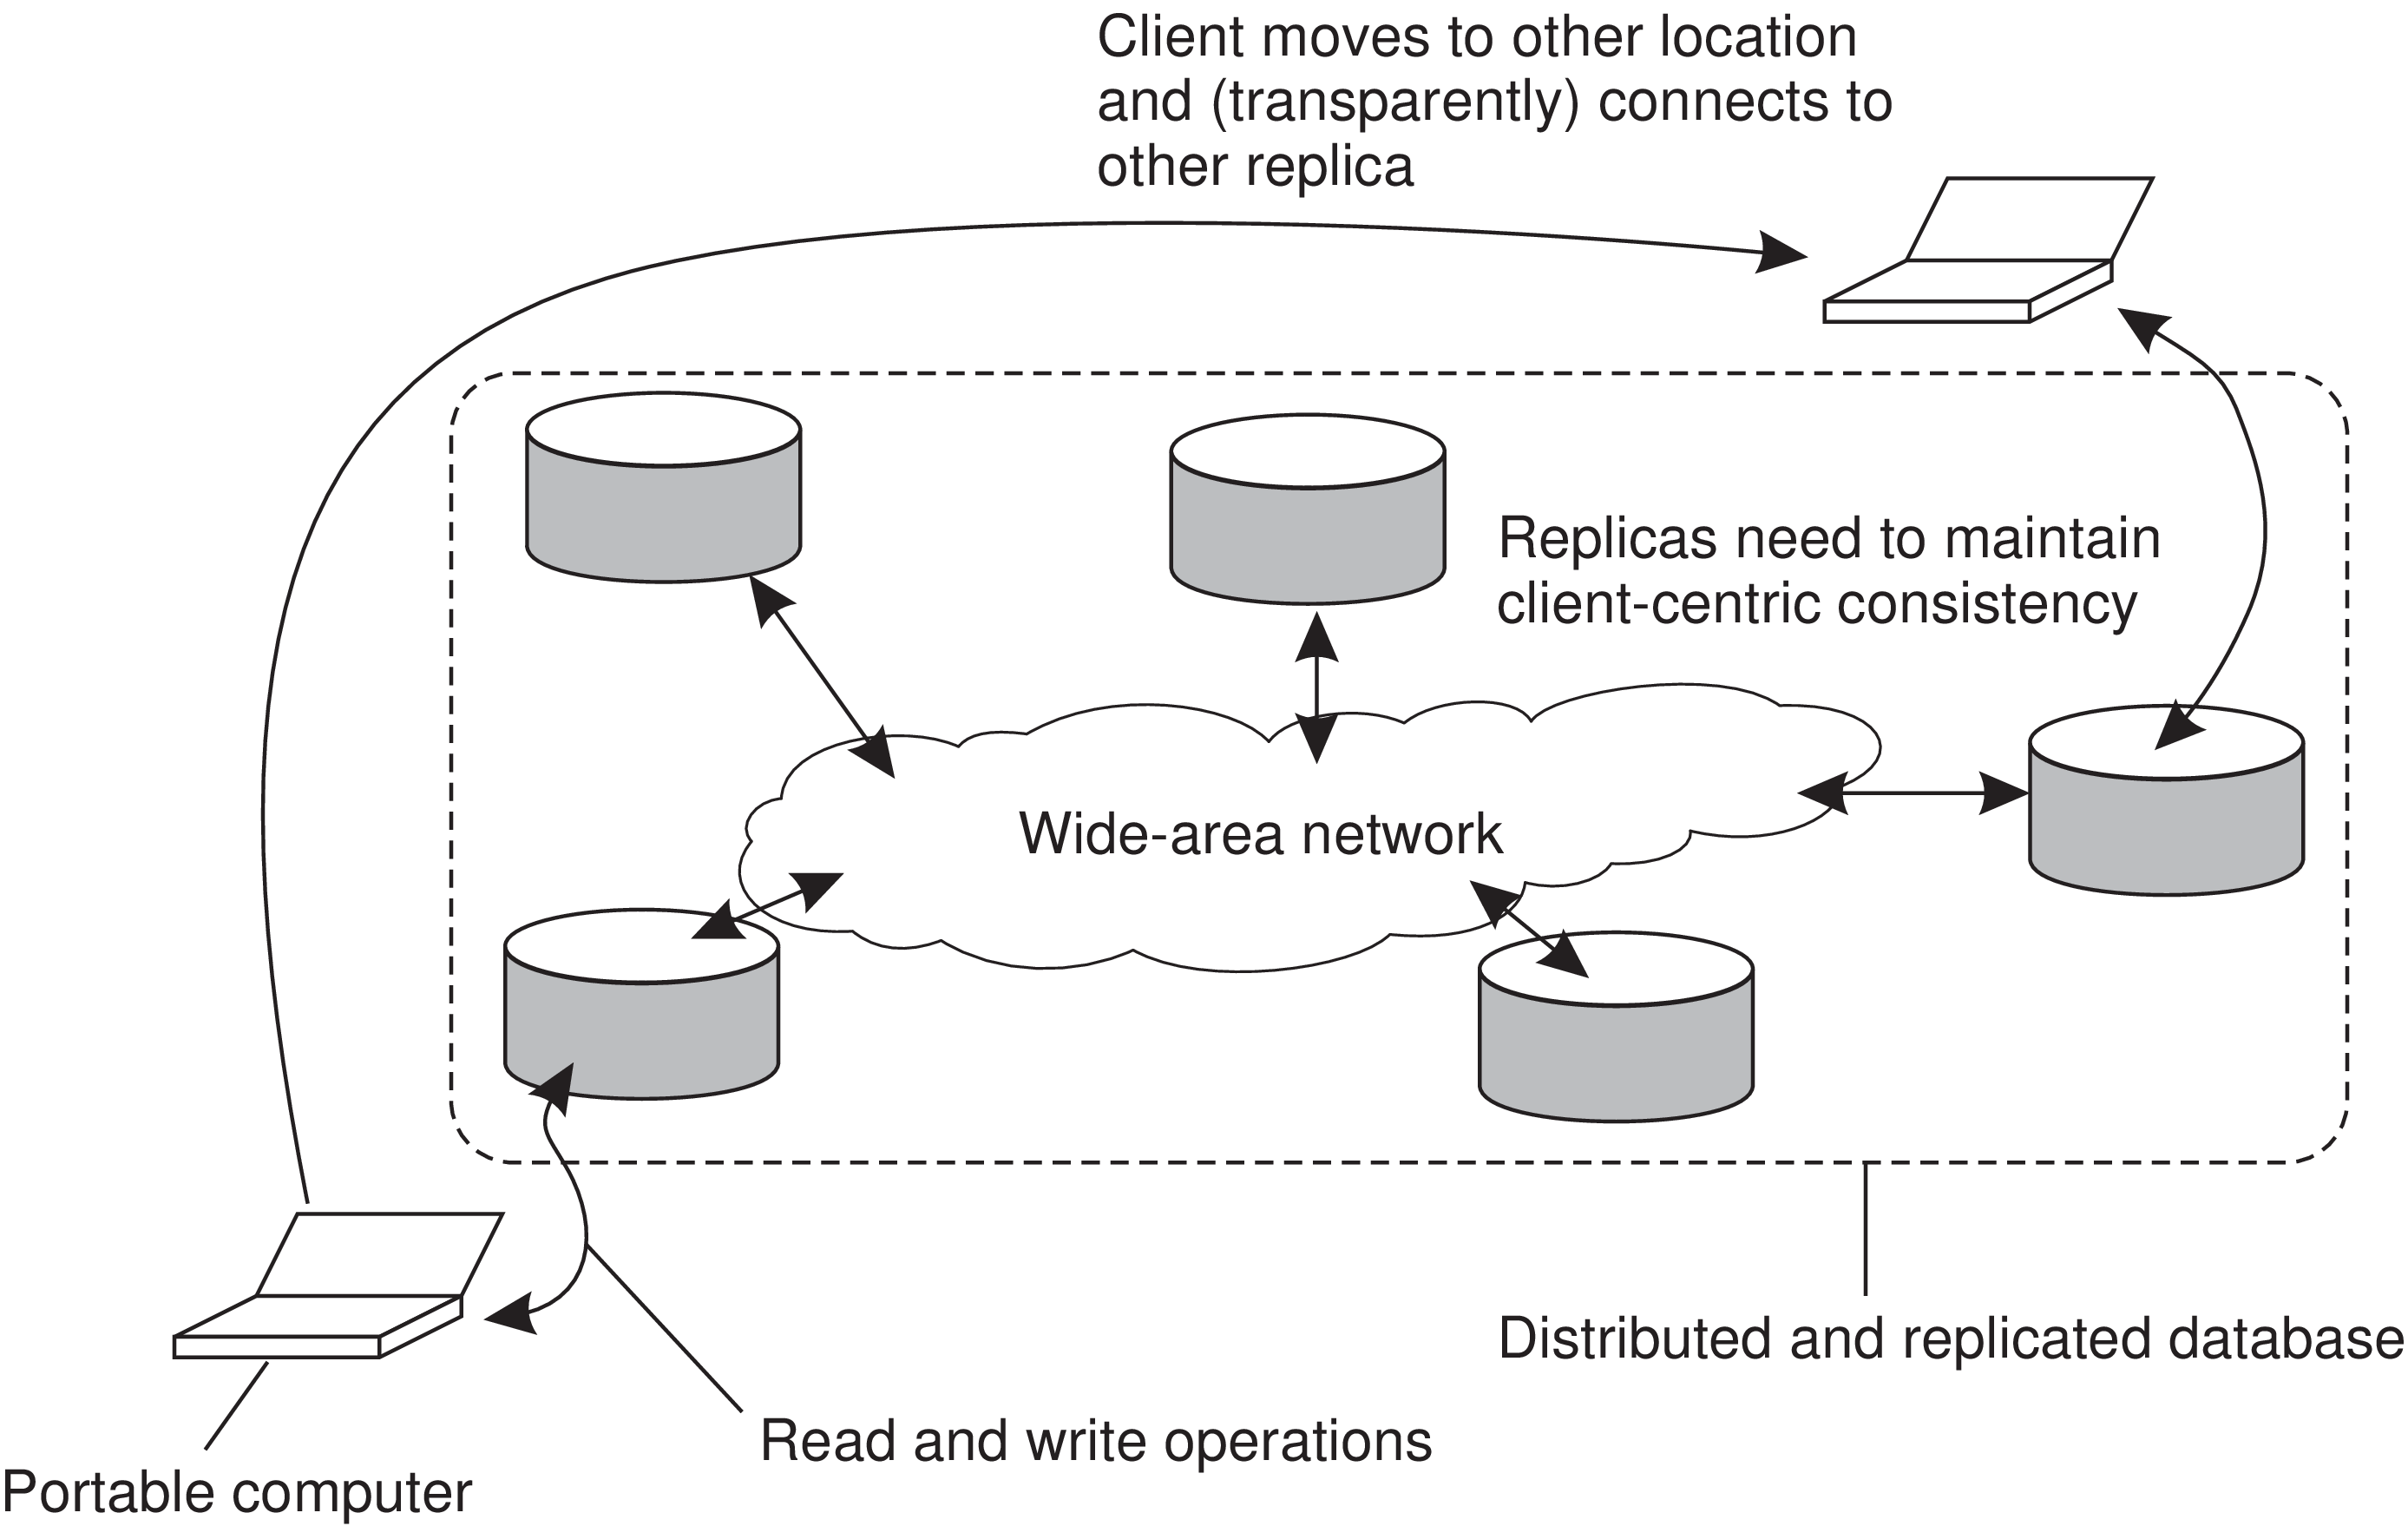
\includegraphics[width=\textwidth]{images/joaozinho.png}

\end{frame}

%% --------------------------------------------------------

\begin{frame}{Notação utilizada}

Vamos usar uma notação um pouco mais elaborada nesta aula
\begin{itemize}
    \item $x_i \leftarrow$ versão do dado $x$
    \item $W_i(x_j) \leftarrow$ processo $i$ está escrevendo no dado $x$
    \item Se temos $x_i$ e $x_j$, sendo $j > i$, dizemos que o dado $x_j$ é mais atualizado
    \begin{itemize}
        \item $W_k(x_i;x_j) \leftarrow$ processo $k$ alterou a versão do dado $x$ de $i$ para $j$
        \item $W_k(x_i|x_j) \leftarrow$ processo $k$ atualizou a versão do dado $x$ de $i$ para $j$ de forma concorrente com outro processo
    \end{itemize}
    \item $R_i(x_j) \leftarrow$ processo $i$ leu a versão $j$ do dado $x$
\end{itemize}
\end{frame}

%% --------------------------------------------------------

\begin{frame}{Leitura monotônica}

Uma coisa importante é garantir a leitura monotônica
\begin{itemize}
    \item Uma leitura posterior de um dado nunca pode retornar uma versão mais antiga
    \item Deve retornar a mesma versão ou então uma mais atualizada
\end{itemize}

\vspace{1cm}

\centering 

Monotônica \hspace{4cm} Não monotônica

\vspace{.15cm}

\centering 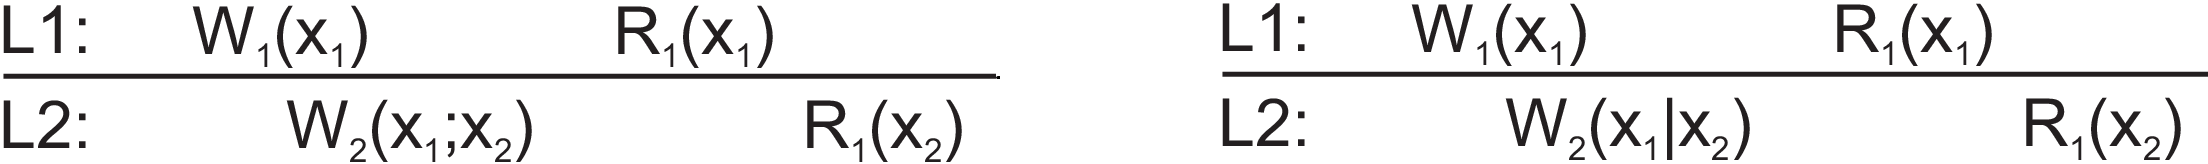
\includegraphics[width=\textwidth]{images/mread.png}
\end{frame}

%% --------------------------------------------------------

\begin{frame}{Escrita monotônica}

Duas atualizações em um dado $x$ por um mesmo processo tem que ser sequenciais
\begin{itemize}
    \item A segunda atualização deve sobrescrever a primeira
    \item Esquema de atualizações FIFO
    \item $W_k(x_i;x_j)$
\end{itemize}

\vspace{1cm}

\centering 

Monotônica \hspace{4cm} Não monotônica

\vspace{.15cm}

\centering 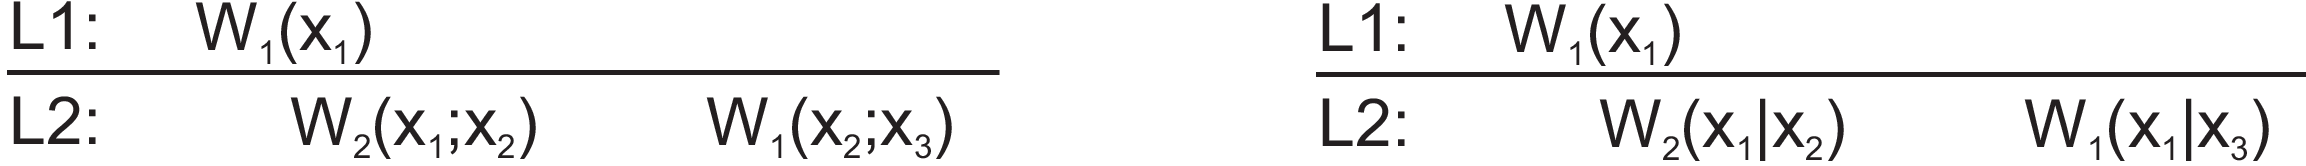
\includegraphics[width=\textwidth]{images/mwrite.png}
\end{frame}

%% --------------------------------------------------------

\begin{frame}{Leia sua escrita}

Uma operação de escrita por um processo $k$ em um dado $x$ deve ser visível a partir de uma requisição de leitura deste mesmo processo (no mesmo dado)
\begin{itemize}
    \item Processo de escrita tem que terminar antes que uma leitura possa ser realizada
\end{itemize}

\vspace{1cm}

\centering 

Consistente \hspace{4cm} Não consistente

\vspace{.15cm}

\centering 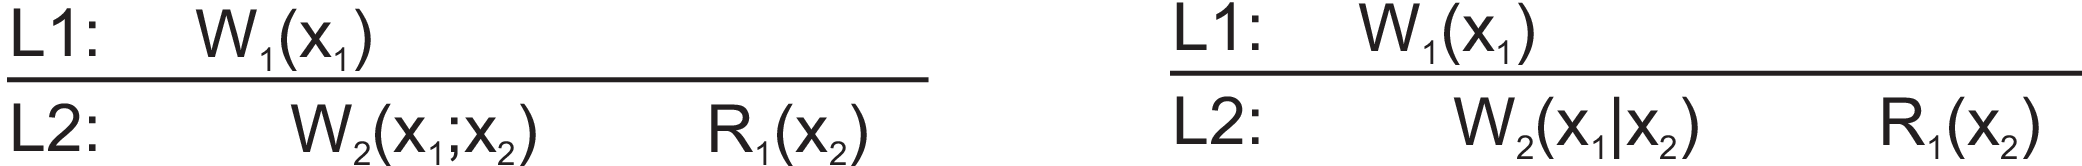
\includegraphics[width=\textwidth]{images/readYwrite.png}

\end{frame}

%% --------------------------------------------------------

\begin{frame}{Escrita segue leitura}

Se um processo $k$ lê um dado $x$ e posteriormente atualiza o valor de $x$ na versão $i$, então este processo de escrita deve ser realizado numa versão $i$ ou mais recente do dado $x$
\begin{itemize}
    \item Uma escrita nunca deve ocorrer sob um dado desatualizado
\end{itemize}

\vspace{1cm}

\centering 

Consistente \hspace{4cm} Não consistente

\vspace{.15cm}

\centering 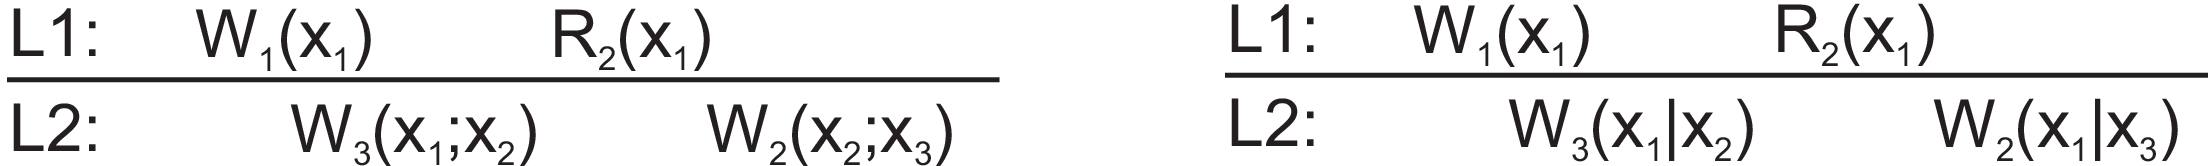
\includegraphics[width=\textwidth]{images/writeFollowRead.png}

\end{frame}

\end{document}
